%--------------------
% Packages
% -------------------
\documentclass[11pt,english]{article}
\usepackage{amsfonts}
\usepackage[left=2.5cm,top=2cm,right=2.5cm,bottom=3cm,bindingoffset=0cm]{geometry}
\usepackage{amsmath, amsthm, amssymb}
\usepackage{tikz}
\usetikzlibrary{calc}
\usetikzlibrary{decorations.pathreplacing,calligraphy}
\usepackage{fancyhdr}
%\usepackage{currfile}
\usepackage{nicefrac}
\usepackage{cite}
\usepackage{graphicx}
\usepackage{caption}
\usepackage{longtable}
\usepackage{rotating}
\usepackage{lscape}
\usepackage{booktabs}
\usepackage{float}
\usepackage{placeins}
\usepackage{setspace}
\usepackage[font=itshape]{quoting}
\onehalfspacing
\usepackage{mathrsfs}
\usepackage{tcolorbox}
\usepackage{xcolor}
\usepackage{subcaption}
\usepackage{float}
\usepackage[multiple]{footmisc}
\usepackage[T1]{fontenc}
\usepackage[sc]{mathpazo}
\usepackage{listings}
\usepackage{longtable}
\definecolor{cmured}{RGB}{175,30,45}
\definecolor{macroblue}{RGB}{56,108,176}
\usepackage[format=plain,
            labelfont=bf,
            textfont=]{caption}
\usepackage[colorlinks=true,citecolor=macroblue,linkcolor=macroblue,urlcolor=macroblue]{hyperref}
\usepackage{varioref}
\usepackage{chngcntr}
\usepackage{datetime}

\definecolor{darkgreen}{RGB}{30,175,88}
\definecolor{darkblue}{RGB}{30,118,175}
\definecolor{maroon}{rgb}{0.66,0,0}
\definecolor{darkgreen}{rgb}{0,0.69,0}

%Counters
\newtheorem{theorem}{Theorem}[section] 
\newtheorem{proposition}{Proposition}
\newtheorem{lemma}{Lemma}
\newtheorem{corollary}{Corollary}
\newtheorem{assumption}{Assumption}
\newtheorem{axiom}{Axiom}
\newtheorem{case}{Case}
\newtheorem{claim}{Claim}
\newtheorem{condition}{Condition}
\newtheorem{definition}{Definition}
\newtheorem{example}{Example}
\newtheorem{notation}{Notation}
\newtheorem{remark}{Remark}


\hypersetup{ 	
pdfsubject = {},
pdftitle = {TidyTuesday Week 7},
pdfauthor = {Pranay Gundam},
linkcolor= macroblue
}


\title{\textbf{TidyTuesday Week 7}}
\author{Pranay Gundam}


%-----------------------
% Begin document
%-----------------------
\begin{document}

\maketitle

\tableofcontents

\section{Weekly Summary}


\section{Date: 2025-02-11}
\noindent \textbf{Series ID: PCU561612561612} 

\noindent This series is titled Producer Price Index by Industry: Security Guards and Patrol Services and has a frequency of Monthly. The units are Index Dec 2004=100 and the seasonal adjustment is Not Seasonally Adjusted.The observation start date is 2004-12-01 and the observation end date is 2024-12-01.The popularity of this series is 3. \\ 

\noindent \textbf{Series ID: CBBCHUSD} 

\noindent This series is titled Coinbase Bitcoin Cash and has a frequency of Daily, 7-Day. The units are U.S. Dollars and the seasonal adjustment is Not Seasonally Adjusted.The observation start date is 2017-12-20 and the observation end date is 2025-02-10.The popularity of this series is 16. \\ 

\subsection{Regression Tables and Plots}
\begin{center}
\begin{tabular}{lclc}
\toprule
\textbf{Dep. Variable:}               & value\_fred\_CBBCHUSD & \textbf{  R-squared:         } &     0.101   \\
\textbf{Model:}                       &          OLS          & \textbf{  Adj. R-squared:    } &     0.090   \\
\textbf{Method:}                      &     Least Squares     & \textbf{  F-statistic:       } &     9.165   \\
\textbf{Date:}                        &    Tue, 11 Feb 2025   & \textbf{  Prob (F-statistic):} &  0.00330    \\
\textbf{Time:}                        &        14:01:41       & \textbf{  Log-Likelihood:    } &   -603.59   \\
\textbf{No. Observations:}            &             84        & \textbf{  AIC:               } &     1211.   \\
\textbf{Df Residuals:}                &             82        & \textbf{  BIC:               } &     1216.   \\
\textbf{Df Model:}                    &              1        & \textbf{                     } &             \\
\textbf{Covariance Type:}             &       nonrobust       & \textbf{                     } &             \\
\bottomrule
\end{tabular}
\begin{tabular}{lcccccc}
                                      & \textbf{coef} & \textbf{std err} & \textbf{t} & \textbf{P$> |$t$|$} & \textbf{[0.025} & \textbf{0.975]}  \\
\midrule
\textbf{const}                        &    1287.7007  &      294.886     &     4.367  &         0.000        &      701.078    &     1874.323     \\
\textbf{value\_fred\_PCU561612561612} &      -6.2375  &        2.060     &    -3.027  &         0.003        &      -10.336    &       -2.139     \\
\bottomrule
\end{tabular}
\begin{tabular}{lclc}
\textbf{Omnibus:}       & 70.902 & \textbf{  Durbin-Watson:     } &     0.375  \\
\textbf{Prob(Omnibus):} &  0.000 & \textbf{  Jarque-Bera (JB):  } &   487.509  \\
\textbf{Skew:}          &  2.606 & \textbf{  Prob(JB):          } & 1.38e-106  \\
\textbf{Kurtosis:}      & 13.589 & \textbf{  Cond. No.          } &  1.20e+03  \\
\bottomrule
\end{tabular}
%\caption{OLS Regression Results}
\end{center}

Notes: \newline
 [1] Standard Errors assume that the covariance matrix of the errors is correctly specified. \newline
 [2] The condition number is large, 1.2e+03. This might indicate that there are \newline
 strong multicollinearity or other numerical problems.

\begin{figure}
\centering
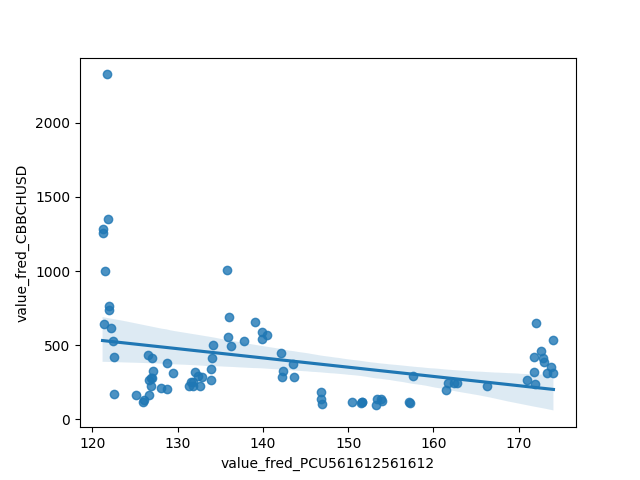
\includegraphics[scale = 0.9]{plots/plot_2025-02-11.png}
\caption{Regression Plot for 2025-02-11}
\end{figure}
\newpage

\include{tex_things/day_2025-02-12}
\include{tex_things/day_2025-02-13}
\section{Date: 2025-02-14}
\noindent \textbf{Series ID: MFSABSNNCB} 

\noindent This series is titled Nonfinancial Corporate Business; Mutual Fund Shares; Asset (DISCONTINUED) and has a frequency of Quarterly, End of Period. The units are Billions of Dollars and the seasonal adjustment is Not Seasonally Adjusted.The observation start date is 1949-10-01 and the observation end date is 2015-01-01.The popularity of this series is 1. \\ 

\noindent \textbf{Series ID: CTFPPPMXA669NRUG} 

\noindent This series is titled Total Factor Productivity Level at Current Purchasing Power Parities for Mexico and has a frequency of Annual. The units are Index USA = 1 and the seasonal adjustment is Not Seasonally Adjusted.The observation start date is 1954-01-01 and the observation end date is 2019-01-01.The popularity of this series is 8. \\ 

\subsection{Regression Tables and Plots}
\begin{center}
\begin{tabular}{lclc}
\toprule
\textbf{Dep. Variable:}          & value\_fred\_CTFPPPMXA669NRUG & \textbf{  R-squared:         } &     0.688   \\
\textbf{Model:}                  &              OLS              & \textbf{  Adj. R-squared:    } &     0.683   \\
\textbf{Method:}                 &         Least Squares         & \textbf{  F-statistic:       } &     132.5   \\
\textbf{Date:}                   &        Fri, 14 Feb 2025       & \textbf{  Prob (F-statistic):} &  7.93e-17   \\
\textbf{Time:}                   &            10:05:40           & \textbf{  Log-Likelihood:    } &    51.299   \\
\textbf{No. Observations:}       &                 62            & \textbf{  AIC:               } &    -98.60   \\
\textbf{Df Residuals:}           &                 60            & \textbf{  BIC:               } &    -94.34   \\
\textbf{Df Model:}               &                  1            & \textbf{                     } &             \\
\textbf{Covariance Type:}        &           nonrobust           & \textbf{                     } &             \\
\bottomrule
\end{tabular}
\begin{tabular}{lcccccc}
                                 & \textbf{coef} & \textbf{std err} & \textbf{t} & \textbf{P$> |$t$|$} & \textbf{[0.025} & \textbf{0.975]}  \\
\midrule
\textbf{const}                   &       1.0423  &        0.017     &    62.588  &         0.000        &        1.009    &        1.076     \\
\textbf{value\_fred\_MFSABSNNCB} &      -0.0023  &        0.000     &   -11.512  &         0.000        &       -0.003    &       -0.002     \\
\bottomrule
\end{tabular}
\begin{tabular}{lclc}
\textbf{Omnibus:}       &  0.144 & \textbf{  Durbin-Watson:     } &    0.212  \\
\textbf{Prob(Omnibus):} &  0.931 & \textbf{  Jarque-Bera (JB):  } &    0.011  \\
\textbf{Skew:}          &  0.032 & \textbf{  Prob(JB):          } &    0.994  \\
\textbf{Kurtosis:}      &  2.986 & \textbf{  Cond. No.          } &     102.  \\
\bottomrule
\end{tabular}
%\caption{OLS Regression Results}
\end{center}

Notes: \newline
 [1] Standard Errors assume that the covariance matrix of the errors is correctly specified.

\begin{figure}
\centering
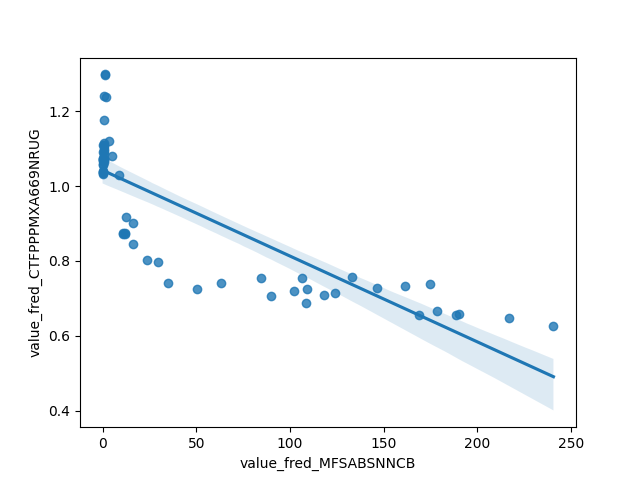
\includegraphics[scale = 0.9]{plots/plot_2025-02-14.png}
\caption{Regression Plot for 2025-02-14}
\end{figure}
\newpage

\include{tex_things/day_2025-02-15}
\include{tex_things/day_2025-02-16}
\include{tex_things/day_2025-02-17}

\end{document}
